% !TEX root=ManualTFG.tex

\chapter{Marc teòric}\label{teoria}

Aquest capítol construeix el marc conceptual necessari per entendre i situar el treball. Abans d'entrar en l'experimentació, cal respondre una sèrie de preguntes prèvies: per què és difícil confiar en una explicació generada per un model, com es pot construir un escenari on la resposta correcta sigui coneguda, amb quins mètodes es generen les explicacions i, finalment, com es mesura si aquestes explicacions són realment fidels al model. Cadascuna d'aquestes preguntes ocupa una part del capítol, i la resposta a cada una motiva la següent. Al final, quan s'hagin introduït les mètriques de qualitat d'imatge i les d'utilitat de l'explicabilitat com a dos mons separats, quedarà plantejat el context teòric que articula tot el treball i podrem reflexionar si tenen alguna cosa a dir les primeres sobre les segones.

\section{Intel·ligència artificial explicable: el problema i el vocabulari}
Durant l'última dècada, els models de \ac{ML} basats en xarxes neuronals profundes han assolit, en nombroses tasques de visió per computador, nivells de rendiment que igualen o superen els dels experts humans. Aquest salt de capacitat, però, ha anat acompanyat d'un augment proporcional de la complexitat interna dels models. Una xarxa convolucional moderna pot contenir desenes de milions de paràmetres ajustats automàticament durant l'entrenament, sense que cap d'ells tingui un significat interpretable de manera aïllada. El resultat és el que la literatura anomena el problema de la \emph{caixa negra}: es disposa d'un sistema que produeix prediccions precises, però del qual no es pot explicar, en termes comprensibles per a una persona, per què ha arribat a una decisió concreta \cite{Adadi2018}.

Aquesta opacitat deixa de ser una qüestió merament tècnica quan els models s'apliquen a dominis on les decisions tenen conseqüències reals, com ara el diagnòstic mèdic, la concessió de crèdits, la justícia predictiva o la conducció autònoma. En aquests contextos, la impossibilitat de justificar una predicció en limita l'adopció, en dificulta l'auditoria i, sota determinats marcs normatius, en compromet directament la legalitat. La necessitat de conciliar el rendiment dels models opacs amb l'exigència de transparència ha donat lloc a un camp de recerca propi, la \ac{XAI}, l'objectiu general de la qual és fer comprensibles per a les persones determinats aspectes d'un sistema d'intel·ligència artificial, ja siguin desenvolupadors, reguladors o usuaris finals.

\subsection{Taxonomia i conceptes clau}
Tot i la maduresa creixent del camp, la \ac{XAI} arrossega una ambigüitat terminològica notable. Termes com ara \emph{explicabilitat}, \emph{interpretabilitat} i \emph{transparència} s'utilitzen sovint de manera intercanviable en una part de la literatura, mentre que en una altra es distingeixen amb matisos precisos \cite{Longo2024}. Aquesta manca de consens dificulta la comparació entre treballs i, en última instància, el progrés ordenat de la disciplina. Per evitar aquesta confusió, en aquest treball s'adopten les distincions que sí que gaudeixen d'un cert acord a la comunitat i que resulten suficients per situar la metodologia emprada.

La primera d'aquestes distincions separa l'explicabilitat \emph{local} de la \emph{global}. Una explicació local justifica una predicció individual del model davant d'una entrada concreta, mentre que una explicació global pretén caracteritzar el comportament del model en conjunt. La segona distingeix entre els models \emph{ante-hoc} i les tècniques \emph{post-hoc}. Els primers són models dissenyats per ser intrínsecament interpretables, com els arbres de decisió o els sistemes basats en regles, en què la transparència forma part de l'arquitectura mateixa; les segones operen sobre un model ja entrenat, possiblement opac, per extreure'n una explicació a posteriori. Dins de les tècniques post-hoc, encara cal una tercera distinció: els mètodes \emph{independents del model} (\emph{model-agnostic}) funcionen sense fer suposicions sobre l'arquitectura subjacent, mentre que els mètodes \emph{específics del model} (\emph{model-specific}) només són aplicables a certes classes de models \cite{Longo2024}. El present treball se situa de manera natural en aquest mapa: s'explica un classificador convolucional ja entrenat mitjançant un mètode post-hoc i local d'atribució de rellevància.

\subsection{Mapes de saliència i el dilema de la intuïció}
Entre les tècniques post-hoc, els mètodes d'atribució de característiques constitueixen una de les famílies més esteses en el domini de la imatge. Aquests mètodes assignen a cada píxel de l'entrada un valor de rellevància que quantifica la seva contribució a la predicció del model, produint una representació visual denominada \emph{mapa de saliència}\footnote{Els mecanismes de càlcul d'aquests valors de rellevància s'expliquen en detall a la secció \ref{sec:metodes}.}. La Figura~\ref{fig:saliency} n'il·lustra un exemple: donat un model de classificació que distingeix entre cans i moixos, i una imatge classificada correctament com a \emph{ca}, el mapa de saliència resultant codifica, píxel a píxel, quina part de l'entrada ha influït més en aquella predicció concreta.

\begin{figure}
\begin{center}
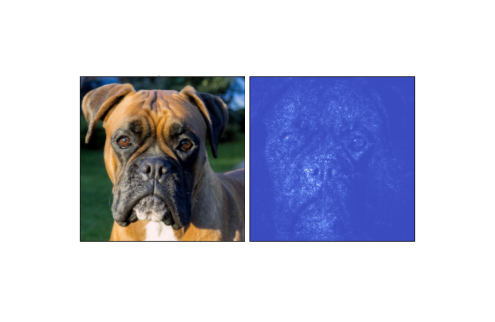
\includegraphics[width=0.9\textwidth]{./figures/teoria/saliency.pdf}
\caption{A l'esquerra, la imatge original d'un ca. A la dreta, el mapa de saliència generat per un mètode d'atribució post-hoc sobre la predicció de la classe \emph{ca}.}
\label{fig:saliency}
\end{center}
\end{figure}

La popularitat d'aquests mètodes es deu, en bona part, a la immediatesa amb què un mapa de rellevància pot ser inspeccionat: davant d'una imatge classificada com a \emph{ca}, resulta intuïtiu comprovar si la rellevància es concentra sobre l'animal o es dispersa sobre regions irrellevants del fons. Cal subratllar, però, una limitació fonamental d'aquesta intuïció: un mapa d'atribució indica \emph{on} mira el model, però no n'explica el \emph{per què}. La interpretació del significat de la regió ressaltada recau sempre sobre la persona que avalua l'explicació, que ha de jutjar si constitueix una evidència vàlida de la classe o no.

Aquesta distància entre allò que un mapa mostra i allò que realment indica sobre el raonament del model s'ha de tenir en compte. Hi ha casos documentats de classificadors que assoleixen una precisió elevada per les raons equivocades, fenòmen conegut com a aprenentatge de dreceres (\emph{shortcut learning}) o, de manera més col·loquial, com a predictors \emph{Clever Hans}. L'exemple canònic és el d'un classificador d'imatges de cavalls que, en lloc d'aprendre a reconèixer l'animal, havia après a detectar una marca d'aigua de copyright present de manera sistemàtica en les imatges d'aquesta categoria \cite{Lapuschkin2019}. El model encertava la predicció, però la seva competència era il·lusòria: depenia d'una correlació arbitrària del conjunt de dades, no de la presència real del cavall. Casos com aquest il·lustren per què l'explicabilitat és una eina necessària per detectar quan un model és fiable i quan no ho és.

Ara bé, perquè una explicació pugui complir aquesta funció diagnòstica, ella mateixa ha de ser de confiança. A diferència de la classificació, on es disposa d'una etiqueta de referència que permet mesurar objectivament l'encert d'una predicció, en l'avaluació de les explicacions no existeix una veritat de referència del que constitueix una explicació \emph{correcta}: si coneguéssim amb certesa quins són els píxels que el model utilitza per decidir, no necessitaríem cap mètode d'atribució per descobrir-los. Aquesta absència de \emph{ground truth} té una conseqüència incòmoda: un mapa de rellevància pot resultar visualment convincent i, alhora, no reflectir el comportament real del model. La plausibilitat per a l'ull humà i la fidelitat respecte al model són propietats independents, i confondre-les pot induir a confiar en explicacions enganyoses. Les seccions següents desenvolupen les eines necessàries per abordar-lo: els models generatius que permeten construir un banc de proves controlat, els mètodes d'atribució emprats i, finalment, les mètriques amb què es mesura tant la qualitat de les imatges com la utilitat de les explicacions.

\section{Models de generació d'imatges sintètiques}
La secció anterior ha conclòs amb un problema obert: sense una veritat de referència, no es pot saber amb certesa si un mapa de saliència reflecteix el raonament real del model o si simplement resulta convincent a la vista. Una manera d'esquivar aquesta limitació consisteix a invertir el plantejament. En lloc de confiar cegament en l'explicació, es pot construir un escenari en què sí que es conegui, per construcció, quina part de la imatge hauria de ser rellevant per a la predicció, i comprovar després si l'explicació s'hi concentra. Aquesta és la idea que vertebra les explicacions \emph{contrafactuals}: davant d'una entrada classificada en una categoria determinada, una explicació contrafactual respon a quin canvi mínim caldria aplicar a l'entrada perquè el model modifiqués la seva decisió.

\subsection{L'enfocament contrafactual}
Portada al domini de la imatge, aquesta idea es materialitza en parells d'imatges que difereixen únicament en una regió controlada com es pot observar en la figura \ref{fig:counterfactual}. A partir d'una imatge original que conté un objecte d'una classe coneguda, es genera una versió \emph{contrafactual} en què l'objecte ha desaparegut, mantenint la resta de l'escena intacta. Si el model és sensible a la presència de l'objecte, la seva predicció hauria de canviar entre les dues imatges, i un mètode d'atribució fiable hauria de localitzar la rellevància precisament sobre la regió que distingeix el parell. El parell contrafactual proporciona, doncs, una aproximació a la veritat de referència que faltava: la regió modificada.

\begin{figure} [h]
\begin{center}
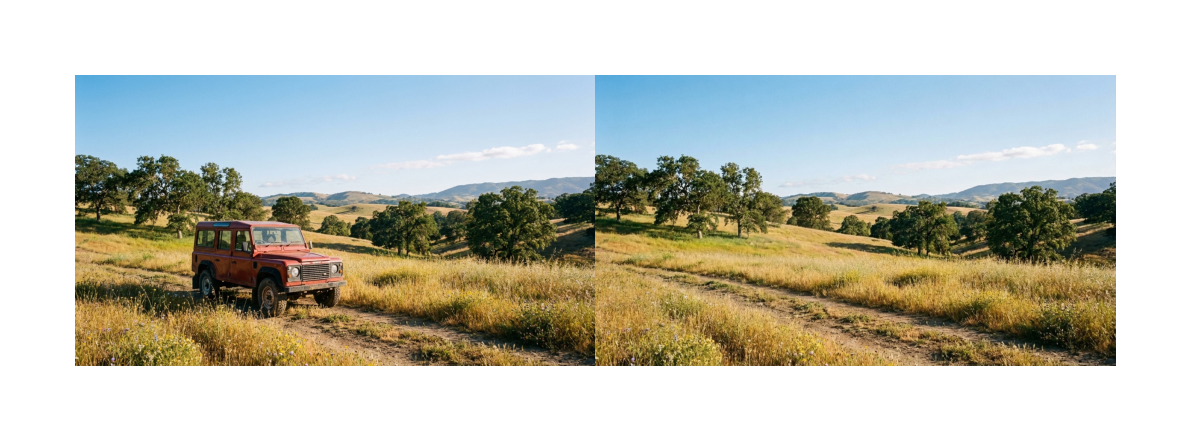
\includegraphics[width=0.9\textwidth]{./figures/teoria/counterfactual.pdf}
\caption{A l'esquerra, la imatge classificada com a \texttt{car=yes}. 
A la dreta, el seu parell contrafactual classificat com a \texttt{car=no}.}
\label{fig:counterfactual}
\end{center}
\end{figure}

La dificultat resideix en com generar aquesta versió contrafactual. L'opció més immediata podria semblar que és esborrar els píxels de l'objecte i deixar-los en blanc o en negre, però és precisament la que s'ha d'evitar. Una regió emmascarada de manera radical és un patró que el model no ha vist mai durant l'entrenament, és a dir, una entrada fora de la distribució de dades. En aquestes condicions, el comportament del model esdevé erràtic i imprevisible, i contamina qualsevol avaluació que se'n derivi. Per obtenir un contrafactual vàlid, s'ha d'agregar o eliminar un objecte i, alhora, reconstruir el fons de manera homogènia, de manera que la imatge resultant continuï pertanyent a la distribució original. Aquesta tasca de reconstrucció coherent d'una regió a partir del seu context s'anomena \emph{inpainting}, i requereix models generatius.

La idea de construir un conjunt de dades plenament controlat per avaluar mètodes d'explicabilitat no és nova. En la recerca feta a \cite{MiroNicolau2026} s'enumeren varis d'ells. Concretament, FunnyBirds \cite{Hesse2023} en constitueix un cas rellevant: hi proposen un conjunt de dades sintètic de renderitzats d'espècies d'ocells artificials, sobre el qual es poden practicar intervencions semànticament significatives com "eliminar un bec" o "afegir una ala" sense provocar canvis de distribució \cite{Hesse2023}. Aquest control total sobre les variables permet una avaluació rigorosa, però s'obté a costa del realisme: les imatges no són fotorealistes, sinó renderitzats artificials d'un domini controlat. Queda obert, doncs, si les conclusions extretes en un entorn tan idealitzat es mantenen quan l'anàlisi es trasllada a imatges naturals, amb la complexitat visual que això comporta.

\subsection{Famílies de models i la tasca d'inpainting}
Els models generatius són sistemes capaços de sintetitzar dades noves que imiten la distribució de les dades amb què s'han entrenat. En el domini de la imatge se'n distingeixen diverses famílies segons l'estratègia de generació. Les \emph{xarxes generatives antagòniques} o \ac{GAN} enfronten dues xarxes en un esquema competitiu: un generador, que produeix imatges noves, i un discriminador, que intenta distingir-les de les reals; l'entrenament prossegueix fins que el generador aconsegueix enganyar sistemàticament el discriminador; StyleGAN n'és un dels exemples més emblemàtics \cite{Karras2019}. Els \emph{models de difusió}, en canvi, es basen en un procés invers: durant l'entrenament s'afegeix renou de manera gradual a una imatge, i una xarxa neuronal aprèn a desfer aquesta degradació pas a pas; en la fase de generació, partint de renou pur, la xarxa el va eliminant progressivament fins a obtenir una imatge nova i coherent \cite{Ho2020}. Actualment constitueixen l'estat de l'art en realisme i diversitat, i Stable Diffusion n'és l'exponent més conegut \cite{Rombach2022}. Finalment, els \emph{models autoregressius} generen la imatge de manera seqüencial, predint cada nou element (píxel o fragment) condicionat als que ja s'han generat, de manera anàloga a com un model de llenguatge prediu cada paraula a partir de les anteriors; DALL·E n'és un exemple representatiu \cite{Ramesh2021}.

L'\emph{inpainting}, en canvi, no constitueix una família de models, sinó una tasca: la de reconstruir una regió absent d'una imatge condicionant-se al context que l'envolta. Qualsevol de les arquitectures anteriors pot abordar-la. És aquesta tasca la rellevant per a l'objectiu del treball, ja que permet modificacions locals i controlades. Concretament, es pot afegir/esborrar un objecte i reconstruir-ne el context/fons sense alterar la resta de l'escena, constituint la base per generar els parells contrafactuals.

Formalment, un model d'\emph{inpainting} rep com a entrada una imatge i una màscara binària que delimita la regió a reconstruir, i en retorna una versió en què aquella regió ha estat reomplerta de manera coherent. La màscara es pot obtenir de dues maneres. La primera és generar-la automàticament amb models de segmentació, com \ac{SAM}\cite{Kirillov2023} o \ac{YOLO}\cite{Redmon2016}, capaços de delimitar objectes arbitraris dins d'una imatge. La segona és aprofitar anotacions ja existents donat un conjunt de dades. Per exemple, un dataset àmpliament usat és \ac{COCO}\cite{Lin2015}, el qual proporciona, per a un gran nombre d'imatges naturals, anotacions de segmentació a nivell d'objecte, cosa que permet seleccionar imatges amb una sola instància de la classe d'interès i emprar-ne directament la màscara associada, evitant els errors que pot introduir una segmentació automàtica.

\begin{figure}
\begin{center}
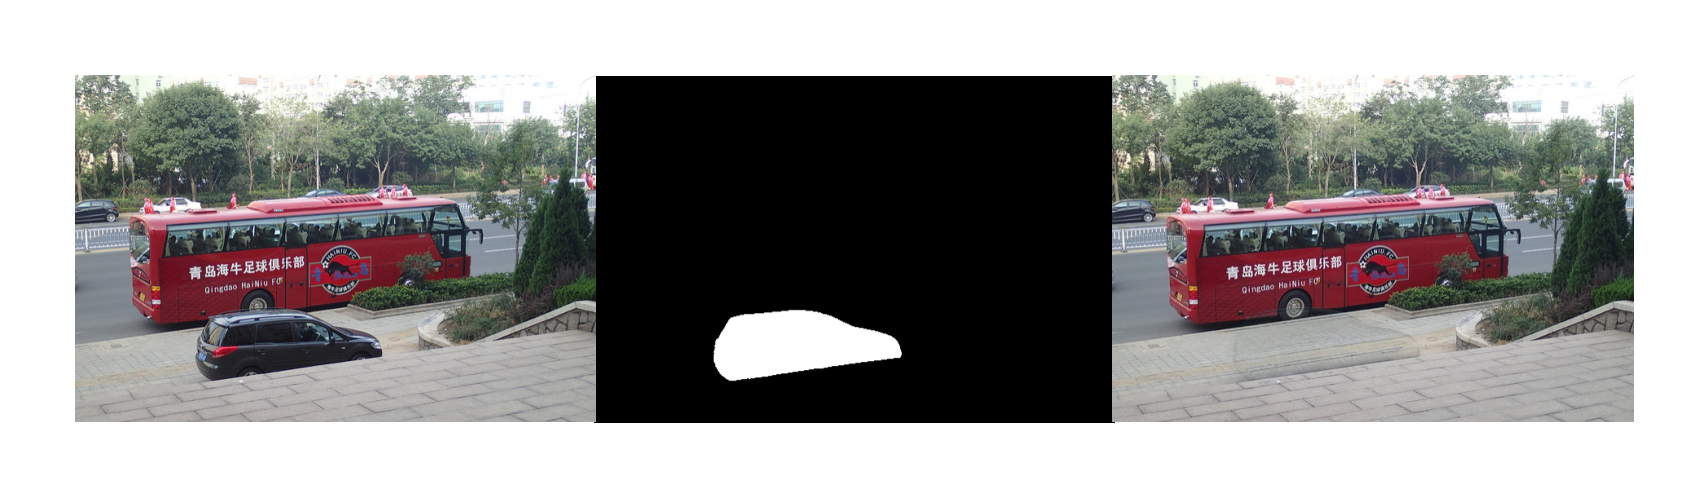
\includegraphics[width=0.9\textwidth]{./figures/teoria/inpainting.pdf}
\caption{Procés de generació d'un parell contrafactual mitjançant \emph{inpainting}. D'esquerra a dreta: imatge original amb l'objecte, màscara binària de la regió a reconstruir i imatge contrafactual resultant, en què l'objecte ha estat eliminat i el fons reconstruït.}
\label{fig:inpainting}
\end{center}
\end{figure}

Dins de la tasca d'\emph{inpainting} hi ha una distinció central per a aquest treball: la de fins a quin punt cada mètode respecta els píxels situats fora de la màscara. Alguns enfocaments hi restringeixen estrictament la seva actuació i preserven la resta de la imatge intacta. D'altres, de naturalesa plenament generativa, poden reinterpretar el context circumdant tenint en compte la il·luminació, les textures o els límits de l'escena, de manera que el contrafactual resultant difereix de l'original no només en l'objecte eliminat, sinó en una porció més àmplia de la imatge. Dos mètodes poden produir, així, contrafactuals igualment convincents a la vista però amb una \emph{empremta de modificació} radicalment diferent. Quins models concrets s'han emprat i les implicacions corresponents es desenvolupen al capítol d'experimentació.

\section{Mètriques de qualitat d'imatge}
Per caracteritzar aquesta empremta de manera objectiva calen mètriques que quantifiquin com i quant difereixen dues imatges. Es tracta d'eines estàndard i d'ús habitual en l'anàlisi d'imatges, i el seu interès recau en el fet que operen a nivells de descripció complementaris, des de la comparació directa de valors de píxel fins a la similitud perceptual d'alt nivell. Les dues primeres treballen sobre els valors de píxel. El \ac{PCP} mesura l'abast espacial de la modificació, és a dir, quina proporció d'una imatge de dimensions $H \cdot W$ s'ha vist alterada:
\begin{equation}
\text{PCP} = \frac{1}{H \cdot W} \sum_{i=1}^{H}\sum_{j=1}^{W} \mathbb{1}\left( \lVert I_{i,j} - I'_{i,j} \rVert > \tau \right) \cdot 100,
\end{equation}
on $\mathbb{1}(\cdot)$ és la funció indicadora i $\tau$ un llindar de tolerància que ignora diferències numèriques insignificants (com les derivades del soroll) i compta només els canvis rellevants. El \ac{PCP} indica, doncs, \emph{quants} píxels han canviat, però no en quina mesura. Aquesta segona informació la proporciona la diferència absoluta mitjana de píxels o \ac{MAPD}, que mesura la intensitat del canvi com la magnitud mitjana de la variació de valor per píxel:
\begin{equation}
\text{MAPD} = \frac{1}{H \cdot W} \sum_{i=1}^{H}\sum_{j=1}^{W} \lVert I_{i,j} - I'_{i,j} \rVert,
\end{equation}
A diferència del \ac{PCP}, que tracta cada píxel de manera binària, el \ac{MAPD} distingeix entre modificacions subtils i dràstiques i ofereix una mesura contínua de la intensitat global. Una en quantifica l'extensió i l'altra la magnitud.

Un nivell més amunt, l'\ac{SSIM} no es basa en la diferència directa de píxels, sinó en propietats perceptuals: compara la luminància, el contrast i l'estructura local de regions corresponents de les dues imatges.
\begin{equation}
\text{SSIM}(I, I') = \frac{(2\mu_I \mu_{I'} + C_1)(2\sigma_{II'} + C_2)}{(\mu_I^2 + \mu_{I'}^2 + C_1)(\sigma_I^2 + \sigma_{I'}^2 + C_2)},
\end{equation}
on $\mu$ i $\sigma$ són la mitjana i la desviació estàndard dels valors de píxel, i $C_1, C_2$ constants de regularització. El seu valor es mou habitualment dins l'interval $[-1, 1]$, on $1$ correspon a dues imatges idèntiques. Pel fet d'avaluar l'estructura i no els valors absoluts, el \ac{SSIM} s'apropa més al judici visual humà i resulta especialment indicat per comprovar si una imatge preserva l'estructura global de l'escena malgrat les modificacions locals introduïdes. En conjunt, les mètriques resumides en la taula \ref{tab:metriques} descriuen l'empremta d'una modificació des d'angles complementaris: l'abast (\ac{PCP}), la intensitat (\ac{MAPD}), i l'estructura (\ac{SSIM}).

\begin{table}
\centering
\begin{tabularx}{\textwidth}{@{} ll X X @{}}
\toprule
\textbf{Mètrica} & \textbf{Nivell} & \textbf{Què quantifica} & \textbf{Interpretació} \\
\midrule
\acs{PCP} & Píxel (abast) & Proporció de píxels alterats per sobre d'un llindar & $[0,1]$. Com més baix, menor és l'abast de la modificació \\
\addlinespace
\acs{MAPD} & Píxel (intensitat) & Magnitud mitjana de la variació de valor per píxel & $\geq 0$. Com més baix, menys intensa és la modificació \\
\addlinespace
\acs{SSIM} & Estructura & Similitud en luminància, contrast i estructura local & $[-1,1]$. Com més alt (proper a 1), més similars són \\
\bottomrule
\end{tabularx}
\caption{Resum comparatiu de les mètriques de qualitat d'imatge considerades, segons el nivell de descripció en què operen i la seva interpretació.}
\label{tab:metriques}
\end{table}

Aquestes mètriques permeten distingir objectivament els dos comportaments descrits abans: un model restringit a la màscara produeix una modificació exterior pràcticament nul·la segons \ac{PCP} i \ac{MAPD}, mentre que un model plenament generatiu hi registra valors no nuls. Ara bé, totes mesuren com de diferents són dues \emph{imatges}, ja sigui a nivell de píxel, d'estructura o de percepció. Si la fidelitat d'imatge que aquestes mètriques quantifiquen prediu la utilitat de les explicacions XAI és, precisament, una reflexió derivada d'aquest treball, i que les seccions següents permetran abordar: primer s'han definir els mètodes que generen aquestes explicacions i, després, les mètriques amb què se'n mesura la fidelitat.

\section{Classificació d'imatges i ResNet-18}
Els parells contrafactuals descrits anteriorment i l'anàlisi d'explicabilitat que es desenvoluparà tot seguit comparteixen un element central: el model de classificació que pren les decisions que es volen explicar. Un model de classificació és un sistema capaç de categoritzar una entrada en alguna de les categories possibles de sortida. Concretament, en el domini de la imatge, l'arquitectura que predomina per a les tasques de classificació és la \ac{CNN}. A diferència d'una xarxa completament connectada, una \ac{CNN} aplica filtres convolucionals que es desplacen al llarg de la imatge i en detecten patrons locals com vores, textures o formes, i els combina de manera jeràrquica: les primeres capes capturen elements simples i les més profundes, conceptes cada pic més abstractes, fins a arribar a objectes sencers. Aquesta estructura, observable en la figura \ref{fig:cnn}, juntament amb la compartició de pesos i les operacions de \emph{pooling} que en redueixen la dimensionalitat, fa que les \ac{CNN} siguin especialment eficients i robustes per a la visió per computador.

\begin{figure}
\begin{center}
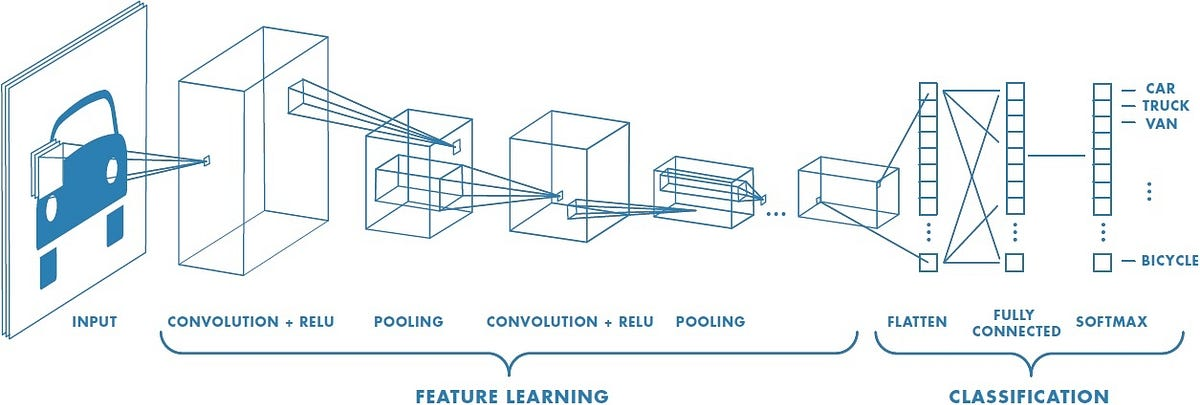
\includegraphics[width=0.9\textwidth]{./figures/teoria/cnn.jpg}
\caption{Estructura arquitectònica d'una \ac{CNN}.}
\label{fig:cnn}
\end{center}
\end{figure}

Durant anys es va assumir que afegir més capes a una xarxa n'augmentaria sempre la capacitat. A la pràctica, però, les xarxes molt profundes pateixen el problema de l'esvaïment del gradient: el senyal d'error es degrada en propagar-se cap a les primeres capes, cosa que en dificulta l'entrenament i, paradoxalment, en pot empitjorar el rendiment. ResNet va resoldre aquest obstacle introduint les connexions residuals: en lloc d'aprendre directament la transformació desitjada, cada bloc aprèn la \emph{diferència} respecte a la seva entrada, que se li torna a sumar mitjançant una connexió de drecera \cite{He2016}. Aquestes dreceres permeten que el gradient flueixi sense degradar-se i fan possible entrenar xarxes de centenars de capes. ResNet-18 n'és una de les variants més lleugeres, amb divuit capes amb pesos, fet que ofereix un bon equilibri entre capacitat i cost computacional.

Entrenar una \ac{CNN} des de zero requereix grans quantitats de dades etiquetades, un recurs que sovint no està disponible per a una tasca concreta. La \emph{transferència d'aprenentatge} ofereix una alternativa: es parteix d'un model ja entrenat en un conjunt de dades gran i general com ImageNet \cite{Deng2009}, que ja ha après representacions visuals útils, i se n'aprofiten els pesos com a punt de partida. A partir d'aquí, l'\emph{ajust fi} reentrena el model sobre les dades de la tasca específica per adaptar-ne les representacions. Aquest pas és especialment rellevant perquè un model genèric, entrenat per a una tasca diferent, no té per què ser sensible a la distinció concreta que es vol estudiar; l'ajust fi és el que el fa reaccionar de manera significativa a la característica d'interès.

En aquest treball, el model que se sotmetrà a anàlisi és un classificador binari basat en ResNet-18, ajustat per distingir la presència o l'absència de l'objecte dins de cada parell contrafactual. La seva funció és doble: d'una banda, ha de ser suficientment sensible a l'objecte perquè la seva predicció canviï entre les dues imatges del parell; de l'altra, és precisament aquest model el que els mètodes d'atribució de la secció següent interrogaran per determinar quines regions de la imatge sustenten les seves decisions.

\section{Mètodes d'atribució}\label{sec:metodes}
En presentar la \ac{XAI} s'ha introduït el concepte de mapa de saliència com a representació visual de la rellevància que un mètode d'atribució assigna a cada píxel. Aquesta secció detalla com es calcula aquesta rellevància. Els mètodes d'atribució es divideixen, a grans trets, en dues famílies segons la manera com sondegen el model \cite{Longo2024}.

\subsection{Aproximacions per pertorbació i gradient}
La primera és la dels mètodes basats en \emph{pertorbació}. La seva idea és alterar sistemàticament l'entrada ocultant o modificant regions i observant com varia la predicció: si amagar una zona fa caure la sortida, aquella zona era important. Hi pertanyen mètodes molt coneguts com LIME\cite{Tulio16}, que aproxima localment el model amb un model interpretable simple, o SHAP, fonamentat en els valors de Shapley de la teoria de jocs. El seu gran avantatge és que són \emph{independents del model}, tractant-lo com una caixa negra. En contrapartida, tenen un cost computacional elevat i, en les seves aproximacions pràctiques, sovint assumeixen independència entre característiques, una hipòtesi que en imatges naturals poques vegades es compleix.

La segona família és la dels mètodes basats en \emph{gradient} o en retropropagació. En lloc de pertorbar l'entrada, aprofiten que la xarxa és diferenciable per propagar informació des de la sortida cap a l'entrada i estimar la contribució de cada píxel. El més elemental és Saliency, que pren directament el gradient de la sortida respecte als píxels d'entrada. Variants posteriors refinen aquesta idea: Deconvolution i Guided Backprop modifiquen la manera de retropropagar el senyal, mentre que Grad-CAM utilitza els gradients respecte a les últimes capes convolucionals per localitzar les regions rellevants. A diferència de la família anterior, aquests mètodes són \emph{específics del model}: requereixen accés als gradients i, per tant, només són aplicables a models diferenciables. A canvi, són molt més eficients, ja que sovint n'hi ha prou amb una sola passada de retropropagació.

El mètode Saliency, però, té una limitació coneguda: la \emph{saturació}. Quan el model ja ha pres una decisió amb confiança, el gradient a l'entrada pot ser pràcticament nul encara que la característica sigui determinant, perquè petites variacions locals ja no n'alteren la sortida. El gradient en un únic punt, doncs, pot infravalorar la importància real d'una característica. És aquí on entra \ac{IG}.

\subsection{Integrated Gradients}
\ac{IG} \cite{Sundarajan2017} substitueix el gradient en un sol punt per la integral dels gradients al llarg d'un camí. La idea és definir una imatge de referència o \emph{baseline} $\mathbf{x}^0$ que representi l'absència d'informació \footnote{En el context de la visió per computador, habitualment una imatge negra.} i recórrer en línia recta des d'aquesta referència fins a la imatge real $\mathbf{x}$, acumulant la sensibilitat de la sortida en cada punt del trajecte. Formalment, l'atribució a la característica $i$ es defineix com:
\begin{equation}
IG_i(\mathbf{x}) = \underbrace{(x_i - x_i^0)}_{\text{canvi}} \cdot \underbrace{\int_0^1 \frac{\partial F\big(\mathbf{x}^0 + \alpha(\mathbf{x} - \mathbf{x}^0)\big)}{\partial x_i}\, d\alpha}_{\text{sensibilitat}},
\end{equation}
on $F$ és la funció que implementa el model i $\alpha$ parametritza el camí entre el \emph{baseline} i l'entrada. L'atribució és, per tant, el producte de dos factors: quant s'allunya la característica del \emph{baseline} (el \emph{canvi}) i quanta sensibilitat acumula la sortida respecte a aquella característica al llarg del camí (la \emph{sensibilitat}). A la pràctica, la integral s'aproxima discretitzant el camí: es generen diverses imatges intermèdies entre el \emph{baseline} i l'entrada, es calcula el gradient de la sortida a cadascuna, se'n fa la mitjana i aquesta mitjana es multiplica, píxel a píxel, per la diferència entre l'entrada i el \emph{baseline}. La Figura~\ref{fig:ig} il·lustra aquest procés.

\begin{figure}
\begin{center}
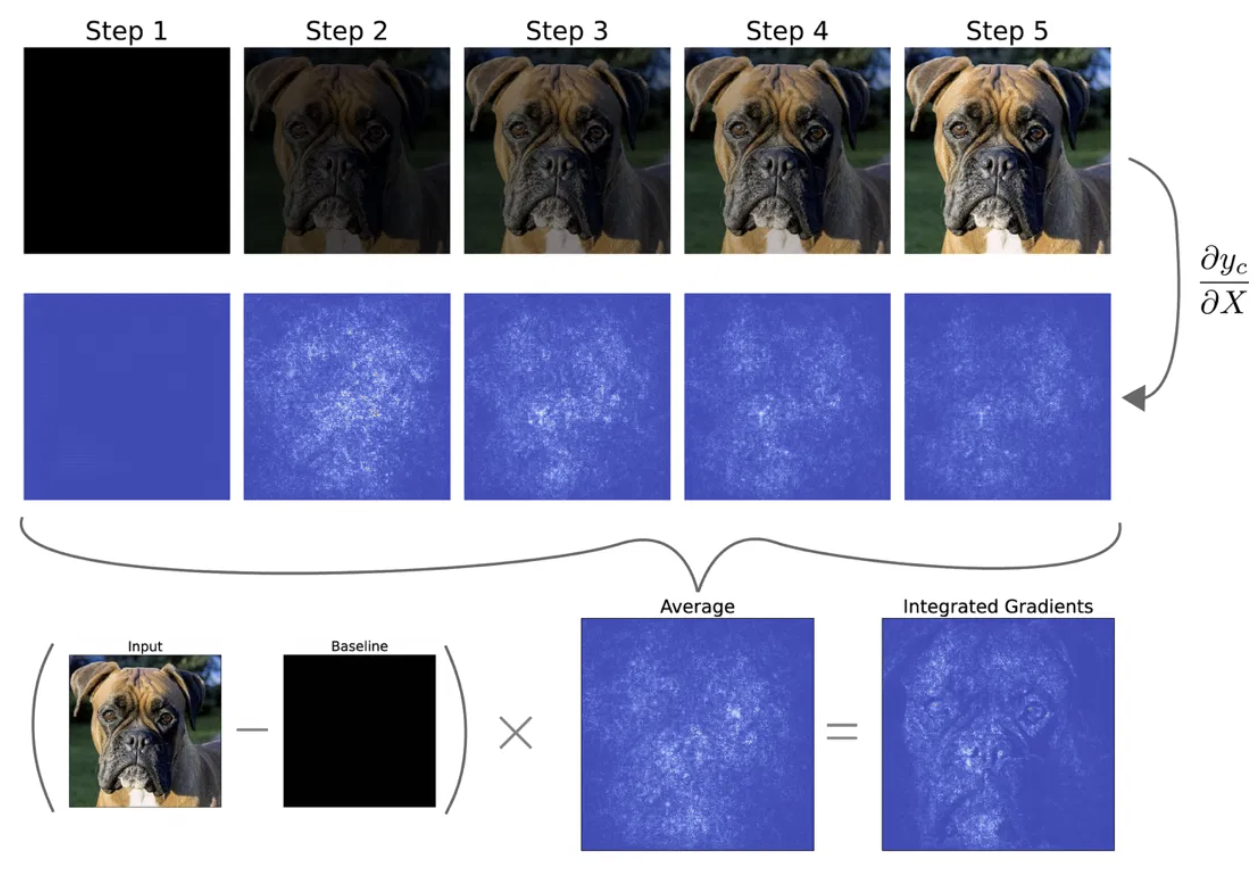
\includegraphics[width=\textwidth]{./figures/teoria/ig.png}
\caption{Procés d'\ac{IG}. A partir de diverses imatges intermèdies entre el \emph{baseline} (imatge negra) i l'entrada, es calculen els gradients a cada pas i se'n fa la mitjana; el resultat es multiplica per la diferència entre l'entrada i el \emph{baseline} per obtenir l'atribució final.}
\label{fig:ig}
\end{center}
\end{figure}

L'interès d'\ac{IG} no resideix només en aquesta construcció, sinó en el fet que no és un mètode \emph{ad hoc}. Abans de proposar-lo, els seus autors es van plantejar quines propietats hauria de complir qualsevol mètode d'atribució per ser fiable, les van formalitzar com a axiomes i, tot seguit, van dissenyar \ac{IG} de manera que els satisfés de forma demostrable \cite{Sundarajan2017}. D'aquests axiomes, dos en constitueixen el nucli. El de \emph{sensibilitat} exigeix que tota característica que influeix en la predicció rebi atribució no nul·la i que, si no hi influeix, en rebi zero; una propietat que, com s'ha vist, els gradients simples poden vulnerar a causa de la saturació. El d'\emph{invariació de l'implementació} exigeix que dos models que calculen la mateixa funció rebin atribucions idèntiques, independentment de com estiguin implementats per dins; \ac{IG} el satisfà perquè depèn únicament dels gradients de la funció, no de la seva arquitectura interna. A aquests s'hi afegeix el de \emph{completitud}: la suma de les atribucions de totes les característiques és exactament $F(\mathbf{x}) - F(\mathbf{x}^0)$, de manera que l'explicació dona compte íntegre de la diferència de predicció entre el \emph{baseline} i l'entrada. Aquestes garanties formals en lloc d'un comportament heurístic distingeixen \ac{IG} de molts altres mètodes d'atribució.

En aquest treball, \ac{IG} i la resta de mètodes d'atribució s'implementen mitjançant Captum \cite{Kokhlikyan2020}, una biblioteca d'interpretabilitat per a PyTorch que en proporciona implementacions de referència. Ara bé, la solidesa axiomàtica que fa atractiu \ac{IG} descriu propietats matemàtiques de l'atribució, però no garanteix per si sola que l'explicació resultant sigui fidel al comportament real del model ni útil per a una persona. Comprovar fins a quin punt aquests mètodes produeixen explicacions fiables exigeix mètriques d'avaluació específiques, que són l'objecte de la secció següent.

\section{Avaluació de l'explicabilitat}
Les seccions anteriors han presentat els mètodes que generen explicacions, però han deixat oberta la pregunta de com saber si una explicació és bona. A diferència de la classificació, on una etiqueta de referència permet mesurar objectivament l'encert, en l'avaluació de l'explicabilitat no existeix una veritat de referència sobre què constitueix una explicació correcta \cite{Longo2024}. Davant d'aquesta absència, la literatura ha proposat descompondre la qualitat d'una explicació en diverses dimensions \cite{Hesse2023}. La més rellevant per a aquest treball és la \emph{fidelitat} (sovint anomenada \emph{correctness}). La fidelitat és el grau en què l'explicació reflecteix el comportament real del model, i no simplement allò que resultaria intuïtiu per a una persona. Una explicació pot ser plausible i, alhora, infidel; per això la fidelitat s'ha de mesurar de manera quantitativa, sense dependre del judici humà.

L'enfocament clàssic per mesurar la fidelitat consisteix a pertorbar l'entrada segons el que diu l'explicació i observar-ne l'efecte sobre la predicció. En el treball de Funnybirds \cite{Hesse2023} per exemple, s'eliminen progressivament parts dels ocells que l'explicació marca com a més rellevants: si l'explicació és fidel, la predicció hauria de caure ràpidament. Aquests protocols, però, arrosseguen un problema fonamental, el mateix que ja s'ha comentat en xerrar de la generació del banc de proves: en emmascarar o alterar píxels es produeix un canvi de distribució que treu la imatge del domini amb què s'ha entrenat el model, de manera que el comportament observat pot ser un artefacte de la pertorbació i no un reflex de la importància real dels píxels. Per això aquesta limitació motiva construir parells contrafactuals dins de distribució mitjançant inpainting d'alta qualitat visual.

Un angle complementari d'avaluació no es pregunta si l'explicació assenyala els píxels correctes, sinó una cosa més bàsica: si l'explicació depèn realment del model. El treball realitzat a \cite{Adebayo2020} es comprova mitjançant tests de randomització: si s'aleatoritzen els pesos del model, una explicació fidel hauria de canviar dràsticament; si no ho fa, és que l'explicació no depèn del que el model ha après. Alguns mètodes d'atribució superen aquesta prova, però d'altres, especialment certes variants de retropropagació, la suspenen i es comporten essencialment com a detectors de vores, ressaltant els contorns de la imatge amb independència del model. Aquest resultat obliga a interpretar amb cautela les explicacions visualment convincents que produeixen aquests mètodes.

\subsection{Mètriques de fidelitat: Focus i caiguda de probabilitat}
Entre les mètriques que avaluen la fidelitat evitant el problema del les imatges fora de distribució destaca el \emph{Focus} \cite{Ariasduart2022}, que s'adopta en aquest treball. En lloc de pertorbar la imatge amb soroll de fora de la distribució, Focus n'introdueix \emph{de dins}: composa mosaics amb imatges de classes diferents i comprova quina proporció de la rellevància que el mètode atribueix cau sobre les imatges de la classe objectiu. La intuïció és que un mètode fidel hauria de concentrar la rellevància sobre les imatges que contenen evidència de la classe. Així, Focus proporciona un estimador quantitatiu i automàtic de la fiabilitat d'un mètode d'atribució, calculat només a partir d'etiquetes d'imatge i sense necessitat d'anotacions a nivell de píxel. A més, és robust als tests de randomització esmentats abans, cosa que en reforça la validesa com a mesura de fidelitat.

Ara bé, malgrat la solidesa axiomàtica d'Integrated Gradients exposada a la secció anterior, els resultats originals de Focus mostren que \ac{IG} produeix explicacions pràcticament aleatòries respecte al model, mentre que mètodes com Grad-CAM o LRP en resulten consistentment fiables \cite{Ariasduart2022}. És a dir, un mètode pot ser impecable des del punt de vista teòric i, alhora, feble quan s'avalua empíricament.

Focus es complementa amb un segon senyal de fidelitat directament lligat al disseny contrafactual: la \emph{caiguda de probabilitat}. Atès que cada parell consisteix en una imatge amb l'objecte i la seva versió sense, una explicació té sentit només si el model és realment sensible a l'objecte; és a dir, si la probabilitat que el model assigna a la classe cau de manera apreciable quan l'objecte s'elimina. Aquesta caiguda mesura, doncs, fins a quin punt la predicció depèn de la regió que distingeix el parell, i permet identificar els casos en què el model no ha reaccionat al canvi i, per tant, es poden estudiar les raons.

\subsection{El nexe entre qualitat visual i fidelitat explicativa}
Arribats a aquest punt, el marc teòric ha posat sobre la taula dues famílies de mètriques que pertanyen a mons diferents. D'una banda, les mètriques de qualitat d'imatge \ac{PCP}, \ac{MAPD} i \ac{SSIM} quantifiquen com de diferents són dues imatges, és a dir, l'empremta de la modificació introduïda pel procés de generació. De l'altra, les mètriques d'utilitat de l'explicabilitat Focus i la caiguda de probabilitat, que quantifiquen fins a quin punt una explicació és fidel al model. Aquestes dues famílies provenen de literatures separades i mesuren coses conceptualment distintes: la primera parla de la imatge i la segona, del que l'explicació revela del model.

Durant el procés de desenvolupament, en la construcció d'un banc de proves contrafactual, és temptador fer servir les mètriques de qualitat d'imatge perquè són àmpliament establertes i fàcils de calcular per validar que la generació és bona i, implícitament, per confiar que els parells així obtinguts donaran lloc a explicacions útils. Però això no garanteix que una imatge contrafactual de gran fidelitat visual produeixi una explicació més fidel al model, ni a la inversa. Verificar el comportament dels mètodes explicatius en prediccions d'un context d'imatges realistes i comprovar si existeix aquesta correspondència entre la qualitat d'imatge i la utilitat de l'explicació són els objectius centrals de l'experimentació que es desenvolupa en el capítol següent.